
\chapter{Linked Queue}

\begin{knowledge}
This part assumes that you have a good understanding of the material on dynamic arrays. 
\end{knowledge}

In this chapter, we'll look at using structs and dynamic memory to make a linked implementation of a queue data type.
A queue is a data structure (sometimes called a FIFO\footnote{\textbf{F}irst \textbf{I}n \textbf{F}irst \textbf{O}ut}) 
where the first item added to the queue is the first one which will come out of the queue.
Contrasted with a stack where the next item to come off the stack is the most recently added.

For this example, we'll make our queue store \texttt{int}s.

\begin{codeinline}
struct queue_node {
    int data;
    struct queue_node* next;
};
\end{codeinline}

Here we have started to define a struct and put a pointer to another struct of the same type inside it.
This is legal in C because as soon the compiler sees \texttt{struct queue\_node}, it will accept mentions of \texttt{struct queue\_node}
as a type. However, while we can do the above, remember that we can't do this:

\begin{codeinline}
struct queue_node {
    int data;
    struct queue_node next;
};
\end{codeinline}
That is, declarare a struct which contains itself (note the lack of pointer).
\footnote{The compiler won't let you actually declare a variable of a 
struct type until it can work out how big it is (which it doesn't know until the closing \}).}



Using this we can have no items in the queue:
\lstinline!struct queue_node* q=0;!
one item in the queue:
\begin{codeinline}
q=malloc(sizeof(struct queue_node));
q->data=7;
\end{codeinline}
or more than multiple items:
\begin{codeinline}
struct queue_node* t=malloc(sizeof(struct queue_node));
t->data=8;
q->next=t;
\end{codeinline}
all via a single pointer variable.
In this case: \lstinline!q->data==7! and \lstinline!q->next->data==8!.

\begin{center}
\scalebox{0.5}{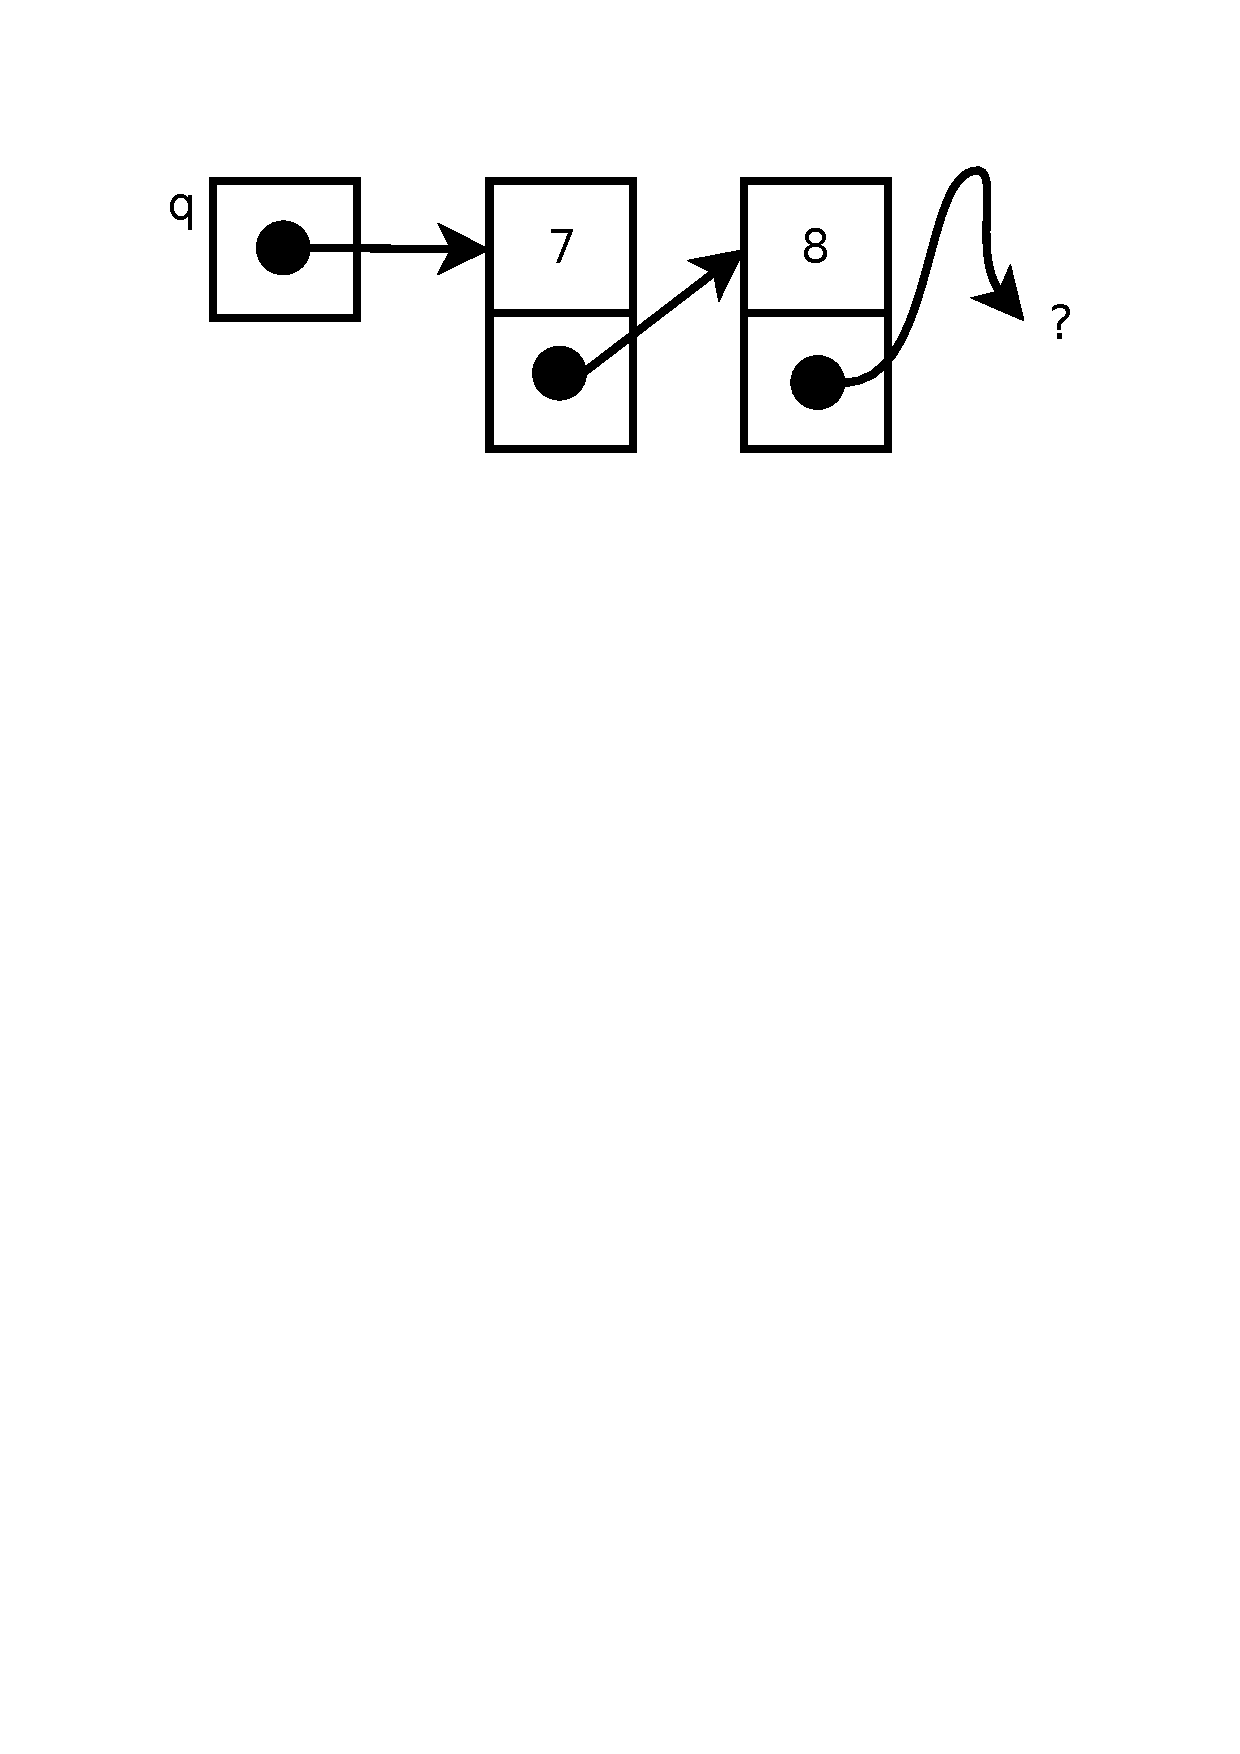
\includegraphics[trim={2.0cm 20.0cm 2.0cm 1.0cm},clip]{queue}}
\end{center}

\emph{Important advice:  drawing pictures is very helpful here. If you are unsure about any code involving pointers, draw a picture.}

If we were sure that the queue had at least 4 items in it, we could write \lstinline!q->next->next->next->data!.
This brings up an important point.
It is critical that the end of linked data structures be properly indicated.
In this case setting the \texttt{next} member to \texttt{0}.
If this ``invariant'' is preserved, you could output all the items in a queue like this:
\begin{codeinline}
struct queue* t=q;
while (t!=0) {
    printf("%d\n", t->data);
    t=t->next;
}
\end{codeinline}

\emph{instruction: stop and make sure you understand exactly what the above does.}

There a number of different visual conventions for indicating a null pointer and it probably doesn't 
matter too much which one you use provided you are consistant. 
Here are some examples:

\begin{center}
\scalebox{0.5}{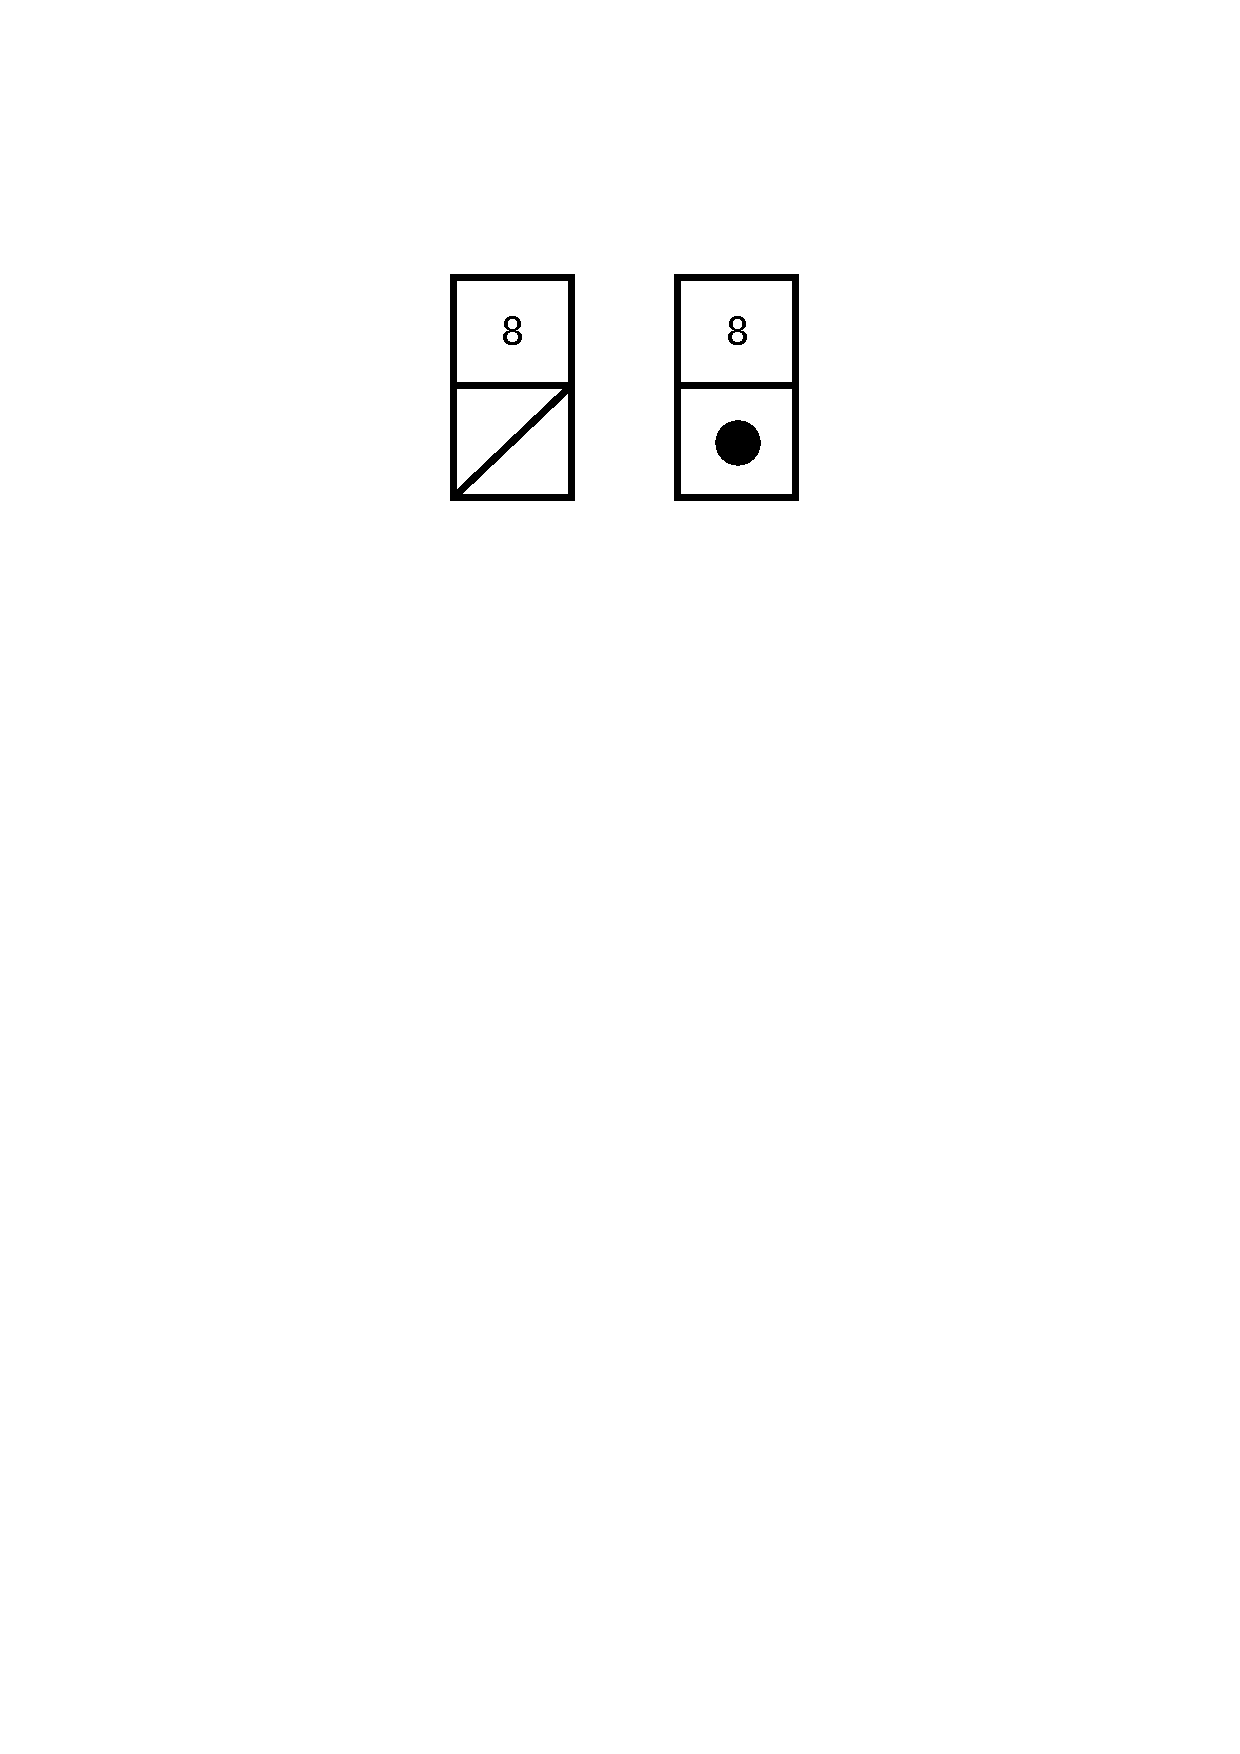
\includegraphics[trim={2.0cm 20.0cm 2.0cm 4.0cm},clip]{nullptr}}
\end{center}



Now we'll add a nicer interface around the queue\_node to make it easier to use.

\begin{codeinline}
struct queue {
    struct queue_node* head;
    struct queue_node* tail;
};
\end{codeinline}

As an optional feature, we could use a \texttt{typedef} to shorten the name.
\begin{codeinline}
typedef struct queue queue;
\end{codeinline}

Since the queue involves memory allocation, we should have setup and teardown/cleanup functions.
\begin{codeinline}
void init_queue(queue* q);
void free_queue(queue* q);
\end{codeinline}
The \lstinline!init_queue()! function assumes that you have already has a queue struct but that it has not been initialised yet.
\begin{codeinline}
queue q;
init_queue(&q);
\end{codeinline}

As an alternative, you could have a function which allocates a queue as well: \lstinline!queue* alloc_queue()!.
Other functions we will need are:
\begin{codeinline}
void add_queue(queue* q, int i);
int get_queue(queue* q);
\end{codeinline}

Notice that this interface doesn't mention malloc even though we know it will be using it.
Let's provide the implementation for these functions.
\begin{codeblock}
void init_queue(queue* q) {
    q->head=0;
    q->tail=0;
}

void free_queue(queue* q) {
    struct queue_node* t=q->head;
    while (t!=0) {
	    // we need this so we can free it
        struct queue_node* temp=t; // after t has moved on
        t=t->next;		
        free(temp);
    }
}
\end{codeblock}

We will add new elements to the end (tail) of the queue and remove items from the front (head) of the queue.
\begin{codeblock}
void add_queue(queue* q, int d) {
      // don't forget the special case of an empty queue
    if (q->head==0) {	
        q->tail=q->head=malloc(sizeof(struct queue_node));
        q->head->next=0;
    } else {
	struct queue_node* n=malloc(
	    sizeof(struct queue_node));
	n->next=0;
	q->tail->next=n
	q->tail=n;
    }
    q->tail->dat=d;
}

int get_queue(queue* q) {
	// check for empty queue first
    if (q->head==0) {
	  // what to do here??
	return 0;
    }
    int result=head->data;
    struct queue_node* temp=q->head;
    q->head=q->head->next;
    free(temp);
      // now we need to check if we have emptied the queue
    if (q->head==0) {
        q->tail=0;
    }
    return result;
}

\end{codeblock}









\section*{Queue summary}
\begin{itemize}
 \item Use structs to carry around all the related variables for a type.
 \item Write setup and cleanup functions for your struct first.
 \item Watch out for special cases.
\end{itemize}
